\section{結果}

\begin{figure*}[h]
  \begin{center}
    \begin{tabular}{c}

      % 1
      \begin{minipage}{0.25\hsize}
        \begin{center}
          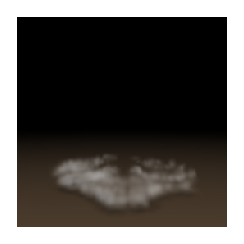
\includegraphics[clip, width=4cm]{./render_20.eps}
          \hspace{1.6cm} (1)20タイムステップ後
        \end{center}
      \end{minipage}

      % 2
      \begin{minipage}{0.25\hsize}
        \begin{center}
          
\includegraphics[clip, width=4cm]{./render_40.eps}
          \hspace{1.6cm} (2)40タイムステップ後
        \end{center}
      \end{minipage}

      % 3
      \begin{minipage}{0.25\hsize}
        \begin{center}
          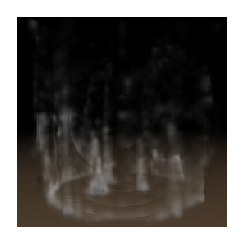
\includegraphics[clip, width=4cm]{./render_60.eps}
          \hspace{1.6cm} (3)60タイムステップ後
        \end{center}
      \end{minipage}

      % 4
      \begin{minipage}{0.25\hsize}
        \begin{center}
          
\includegraphics[clip, width=4cm]{./render_80.eps}
          \hspace{1.6cm}  (4)80タイムステップ後 
        \end{center}
      \end{minipage}  

    \end{tabular}
    \caption{湯気のシミュレーションのレンダリング結果}
    \label{result}
  \end{center}
\end{figure*}


湯気のシミュレーションのレンダリング結果を図(\ref{result})に示す.
格子法と粒子法を用いることで,格子法のみでは実現が困難な水滴の発生位置による微細な湯気の動きを再現した.
本レンダリング結果では湯気の発生分布が大きく2つに分かれている様子を確認した.
レンダリングは格子ごとに湯気の密度を合計し,ボリュームレイキャスティング法により行った.
シミュレーション空間は32×32×32の格子で,シミュレーションで発生した粒子数は3,000個から4,000個となった.
計算時間はIntel Core i5-6200U 2.3GHzのCPUを用いて1タイムステップあたり3秒から4秒となった